% ============================================================
%  CROWS — Combat Robot Optimized Weapon Spinner
%  Research Poster  |  A0 Landscape  |  4 columns
%  Flow: Introduction → Methodology → Parameterisation →
%        Objectives/Evaluation → Stability → ROM → Conclusion
%  Style: TAMU Engineering — maroon header, white content,
%         burnt-orange section headings, clean column dividers
% ============================================================
\documentclass[final]{beamer}
\usepackage[size=a0,orientation=landscape,scale=1.0]{beamerposter}
\usepackage{amsmath,amssymb}
\usepackage{graphicx}
\usepackage{booktabs}
\usepackage{array}
\usepackage{tabularx}
\usepackage{xcolor}
\usepackage{microtype}
\usepackage{multirow}
\usepackage{ragged2e}
\usepackage{tikz}

% ---- Color palette ----
\definecolor{tamumaroon}{RGB}{80,0,0}
\definecolor{tamugold}{RGB}{191,87,0}
\definecolor{pagebg}{RGB}{240,240,240}
\definecolor{colsep}{RGB}{160,160,160}
\definecolor{darktext}{RGB}{20,20,20}

% ---- Strip beamer blocks to plain headings ----
\usetheme{default}
\setbeamertemplate{navigation symbols}{}
\setbeamersize{text margin left=0cm,text margin right=0cm}
\setbeamercolor{background canvas}{bg=pagebg}
\setbeamercolor{block title}{fg=tamugold,bg=white}
\setbeamercolor{block body}{fg=darktext,bg=white}
\setbeamerfont{block title}{size=\large,series=\bfseries}
\setbeamerfont{block body}{size=\small}

\setbeamertemplate{block begin}{%
  \vskip1.8ex
  {\usebeamerfont{block title}\usebeamercolor[fg]{block title}%
   \underline{\insertblocktitle}}\par\vskip0.6ex}
\setbeamertemplate{block end}{\vskip0.4ex}

\setbeamercolor{block title alerted}{fg=tamumaroon,bg=white}
\setbeamercolor{block body alerted}{fg=darktext,bg=white}
\setbeamertemplate{block alerted begin}{%
  \vskip1.8ex
  {\usebeamerfont{block title}\usebeamercolor[fg]{block title alerted}%
   \underline{\insertblocktitle}}\par\vskip0.6ex}
\setbeamertemplate{block alerted end}{\vskip0.4ex}

% ---- Headline ----
\setbeamertemplate{headline}{%
  \leavevmode
  \begin{beamercolorbox}[wd=\paperwidth,ht=9.5cm,dp=0.2cm]{tamuheader}%
    \vbox to 9.5cm{\vfil
      \hbox to \paperwidth{%
        \hspace{0.55cm}%
        \parbox[c][6.5cm][c]{0.19\paperwidth}{\centering
          \includegraphics[height=6.5cm,keepaspectratio]{assets/tamu-engr-logo.png}}%
        \hfill
        \begin{minipage}[c]{0.50\paperwidth}
          \centering
          {\color{white}\fontsize{64}{72}\selectfont\bfseries
            Combat Robot Optimized\\[0.2cm]Weapon Spinner (CROWS)}\\[0.5cm]
          {\color{white}\fontsize{28}{34}\selectfont\bfseries Ian Wilhite}
        \end{minipage}%
        \hfill
        \parbox[c][6.5cm][c]{0.19\paperwidth}{\centering
          \includegraphics[height=6.5cm,keepaspectratio]{assets/roving_robotics_logo-nobg.png}}%
        \hspace{0.55cm}%
      }%
    \vfil}%
  \end{beamercolorbox}%
}
\setbeamercolor{tamuheader}{fg=white,bg=tamumaroon}

% ---- Column dividers ----
\setbeamertemplate{background}{%
  \begin{tikzpicture}
    \useasboundingbox (0,0) rectangle (\paperwidth,\paperheight);
    \foreach \xfrac in {0.250,0.500,0.750} {
      \draw[color=colsep,line width=0.6pt]
        (\xfrac\paperwidth, \paperheight-10.0cm)
        -- (\xfrac\paperwidth, 2.2cm);
    }
  \end{tikzpicture}%
}

% ---- Footline ----
\setbeamertemplate{footline}{%
  \begin{beamercolorbox}[wd=\paperwidth,ht=1.8cm,dp=0.3cm,center]{tamuheader}
    {\color{white}\normalsize
      Weapon Designer Optimization Framework
      $\;\cdot\;$ Texas A\&M University
      $\;\cdot\;$ 2026 $\;\cdot\;$
      \texttt{github.com/Ian-Wilhite/weapon-designer}}
  \end{beamercolorbox}%
}

% ---- Helpers ----
\newcolumntype{Y}{>{\raggedright\arraybackslash}X}
\emergencystretch=3em
\tolerance=9999
\hbadness=9999
\newcommand{\compactlist}{%
  \setlength{\itemsep}{1pt}\setlength{\parskip}{0pt}%
  \setlength{\topsep}{2pt}\setlength{\leftmargin}{1.2em}}

% ============================================================
\begin{document}
\begin{frame}[t]{}

\vskip0.3cm
\begin{columns}[t,totalwidth=\paperwidth]
\begin{column}{0.015\paperwidth}\end{column}

% ============================================================
%  COLUMN 1 — Introduction + Methodology
% ============================================================
\begin{column}{0.220\paperwidth}

\begin{block}{Introduction}
{\centering\includegraphics[width=0.75\linewidth]{assets/robot_photo.png}\\[0.3ex]}
{\footnotesize\centering\textit{Fig.~1:} Battlebots Champion ``Bite Force'' using a vertical spinner.\par}

  \medskip
  
  In combat robotics, spinning weapons store kinetic energy before each impact.
  Across hobby weight classes (1\,lb antweight to 30\,lb featherweight),
  weapon masses range 0.1--4\,kg at 3{,}000--12{,}000\,RPM,
  storing $50$--$10{,}000$\,J per hit.

  \medskip
  Current practice relies on \textbf{empirical design rules}:
  wall-thickness proxies, manual iteration, and build-and-break testing.
  No principled framework simultaneously trades off geometry, structural
  safety, and engagement quality.

  \medskip
  \textbf{CROWS} closes this gap with a modular optimization pipeline:
  physics-based objectives, 2D FEA-in-loop, and a GP surrogate for
  fast design screening.

\end{block}

\begin{block}{System Architecture}
\textbf{Five independently swappable optimization slots:}

\medskip
\resizebox{\linewidth}{!}{%
\begin{tabular}{@{}lll@{}}
\toprule
\textbf{Slot} & \textbf{Options} & \textbf{Config key} \\
\midrule
Outer profile   & Fourier; B-spline; B\'ezier; Catmull-Rom & \texttt{profile\_type} \\
Interior voids  & Superellipse pockets; SIMP topology        & \texttt{cutout\_type} \\
Objective       & Baseline (formula); enhanced (spiral+FEA) & \texttt{eval\_mode} \\
Normalisation   & None; robust rolling IQR              & ---\\
Eval gate       & Off; staged (geom / cheap / FEA)      & \texttt{staged\_gate} \\
\bottomrule
\end{tabular}}

\medskip
\textbf{Design requirements:}
\begin{itemize}\compactlist
  \item Maximise $\tfrac{1}{2}I\omega^2$ within mass \& envelope budget
  \item Maximise kinematic bite depth per tooth engagement
  \item Safety factor $\mathrm{SF}\!\geq\!1.5$ under centrifugal + contact loads
  \item CoM offset $\leq\!3\%$ of $R_{\max}$ (dynamic balance)
\end{itemize}
\end{block}




\begin{block}{Profile Parametrisation Methods}
Five families map $N{=}12$ control radii to a closed boundary polygon.
\textbf{Fourier radial} (baseline) and \textbf{periodic B-spline} (C$^2$)
suffer global support and ill-conditioned Jacobians
($\kappa{\sim}10^5$ and $10^{12}$ respectively), causing parameter
directions invisible to gradient-free mutation.
\textbf{Composite Bézier} and \textbf{centripetal Catmull-Rom} (both C$^1$)
achieve local support, full rank, and $\kappa{<}100$;
Catmull-Rom interpolates control points exactly, enabling
archetype warm-starts.

\medskip
\includegraphics[width=\linewidth]{assets/profile_comparison.png}

{\footnotesize
\textit{Fig.~2:} All five families on a 3-lobe eggbeater
($N{=}12$, $r_i{=}60{+}22\cos 3\theta_i$\,mm).
Orange dots = control points; Catmull-Rom passes through each exactly.
$\kappa(J)$ annotated per panel; B-spline and Fourier show elevated condition.}
\end{block}





\end{column}

\begin{column}{0.030\paperwidth}\end{column}

% ============================================================
%  COLUMN 2 — Parameterisation Methods
% ============================================================
\begin{column}{0.220\paperwidth}


\begin{block}{Functional Harmonic Parametrisation}
\textbf{Radial harmonic series (6 parameters):}
\begin{equation}
  r(\theta) = R_0
  + A_1\cos\!\bigl(n(\theta{-}\phi)\bigr)
  + A_2\cos\!\bigl(2n(\theta{-}\phi)\bigr)
  + A_3\cos\!\bigl(3n(\theta{-}\phi)\bigr)
\end{equation}

\medskip
\textbf{Analytic seeding from bite target:}
\begin{equation}
  n^* = \frac{(v/\omega)\cdot 2\pi}{b_{\text{target}}}
\end{equation}

\medskip
\textbf{Two-stage functional optimizer:}\\
\textit{Stage A} --- 6-dim DE in $\{n,R_0,A_1,A_2,A_3,\phi\}$,
\texttt{popsize=20}.  Rapidly explores the interpretable harmonic manifold.\\
\textit{Stage B} --- lifts to $N{=}12$ B-spline control radii
warm-started from Stage~A's lobed solution; proximity penalty
$\lambda\|\mathbf{r}-\mathbf{r}_{\mathrm{ref}}\|^2$ anneals
($\lambda$ halved every stagnation plateau) allowing refinement
beyond the harmonic manifold while preserving physical intent.
\end{block}


\begin{block}{Optimization \& Evaluation Criteria}
\textbf{Baseline weakness 1 --- Formula bite:}
$b=v/(n_{\text{teeth}}\,f_{\text{rot}})$, $n_{\text{teeth}}$
hardcoded per weapon style.  Optimizer \emph{cannot} reward
sharp geometry.

\medskip
\textbf{Kinematic Archimedean spiral bite:}
opponent traces
$r_{\text{enemy}}(\theta)=r_{\text{start}}-(v/\omega)\,\theta$.
Count zero-crossings with weapon profile per revolution:
\begin{equation}
  b_{\text{eff}} = \frac{(v/\omega)\cdot 2\pi}{n_{\text{contacts}}}
\end{equation}
Smooth disk: $n_c{=}1$,\; $b_{\text{eff}}{\approx}1.7$\,mm.
Twelve teeth: $n_c{\approx}12$,\; $b_{\text{eff}}{\approx}0.14$\,mm.

\medskip
\includegraphics[width=\linewidth]{assets/spiral_contact.png}

{\footnotesize
\textit{Fig.~3:} Archimedean spiral overlays on smooth disk (left)
and 3-tooth weapon (centre).  Right: bite-depth polar roses.
Max bite 1.7\,mm (smooth) vs.\ 45.7\,mm (toothed).
Contact normal $\rightarrow$ FEA point-force loading.}

\medskip
\textbf{2D CST FEA-in-loop} (${\approx}15$\,ms/call, $\Delta x{=}10$\,mm):
\begin{equation}
  \boldsymbol{f}_c=\rho\omega^2\boldsymbol{r},\quad
  \mathrm{SF}=\frac{\sigma_{\text{yield}}}{\sigma_{\text{VM,max}}},\quad
  \mathrm{SF}{<}1.5\;\Rightarrow\;E_{\text{score}}=0
\end{equation}

\textbf{Energy transfer objective:}
\begin{equation}
  E_{\text{transfer}}=
  \underbrace{\tfrac{1}{2}I\omega^2}_{\text{KE}}
  \cdot\underbrace{\cos^2\!\theta_c}_{\text{normal vel.}^2}
  \cdot\frac{b_{\text{eff}}}{b_{\text{max}}},
  \quad E_{\text{score}}=\frac{E_{\text{transfer}}}{E_{\text{ref}}}
\end{equation}

\medskip
\textbf{FEA In-Loop --- Optimization History (Heavyweight Disk):}

\medskip
\includegraphics[width=\linewidth]{assets/fea_training_cycle.png}

{\footnotesize
\textit{Fig.~4:} Von-Mises stress maps at DE steps 1, 20, 40, 60, 67
(B-spline profile, 8{,}000\,RPM, AR500 $\sigma_y{=}1{,}400$\,MPa,
colour normalised to yield).
Profile evolves toward higher-MOI lobe geometry while avoiding
stress concentrations at the bore and pocket boundaries.}
\end{block}

\end{column}

\begin{column}{0.030\paperwidth}\end{column}

% ============================================================
%  COLUMN 3 — Objectives / Evaluation + Stability Analysis
% ============================================================
\begin{column}{0.220\paperwidth}


\begin{block}{Interior Weight-Relief Cutouts}
\textbf{Phase~2 superellipse pockets} remove surplus mass while
preserving structural integrity:
\begin{equation}
  \left|\frac{x'}{a}\right|^n + \left|\frac{y'}{b}\right|^n \leq 1,
  \quad
  (x',y') = R_\phi\bigl(x-r\cos\phi,\;y-r\sin\phi\bigr)
\end{equation}
Parameters $(r,\phi,a,b,n)$: radial distance, angular position,
semi-axes, shape exponent.

\medskip
\textbf{Topology optimisation (SIMP)} --- alternative Phase~2:
\begin{equation}
  E_{\mathrm{eff}}(\rho)=E_{\min}+\rho^p(E_0-E_{\min}),\quad p{=}3
\end{equation}
OC update minimises compliance minus weighted MOI under
$\Sigma\rho_e A_e/A_{\mathrm{total}}=V_f$.
Density-filter radius $r_{\min}{=}2.5\,\Delta x$ suppresses
checkerboard artefacts; hub and rim strips held solid.

\medskip
\textbf{FEA Solver Verification (Lam\'e analytical solution):}

\medskip

\includegraphics[width=\linewidth]{./assets/fea_verification.png}

{\footnotesize
\textit{Fig.~5:} Von-Mises field, per-element vs.\ Lam\'e profile,
and error summary on a solid disk (8{,}000\,RPM, AR500).
Errors ${<}2\%$ at $r{=}0.5R$; ${<}15\%$ at $r{=}0.7R$.
The 2D plane-stress CST mesh captures centrifugal stress
accurately at combat-relevant speeds.}
\end{block}

\begin{block}{Stability Analysis --- Profile Jacobian}
Decompose $dO/d\boldsymbol{x}=J^\top\boldsymbol{q}$,\quad
$J=\partial\boldsymbol{p}/\partial\boldsymbol{x}\in\mathbb{R}^{360\times N}$.
Low $\kappa(J)$ $\Leftrightarrow$ uniform sensitivity: each control-point
mutation moves the weapon boundary predictably.

\medskip
\resizebox{\linewidth}{!}{%
\begin{tabular}{@{}lccrrr@{}}
\toprule
\textbf{Family} & \textbf{Cont.} & \textbf{Local?} &
$\kappa(J)$ & rank & $\bar{c}$ \\
\midrule
PW-linear   & C$^0$      & Yes   & 95                    & 12/12 & 1.000 \\
Fourier     & C$^\infty$ & No    & $1.1{\times}10^{5}$   & 10/12 & 1.000 \\
B-spline    & C$^2$      & Part. & $6.8{\times}10^{12}$  &  9/12 & 0.848 \\
B\'ezier      & C$^1$      & Yes   & 76                    & 12/12 & 1.000 \\
Catmull-Rom & C$^1$      & Yes   & 96                    & 12/12 & 1.000 \\
\bottomrule
\end{tabular}}

\smallskip
{\footnotesize
$\bar{c}$: gradient direction consistency across step sizes (1.0 = ideal).
$\kappa{\sim}10^{13}$ for B-spline is \textbf{structural} --- persistent
for all $N\in\{4,\ldots,20\}$.}

\medskip
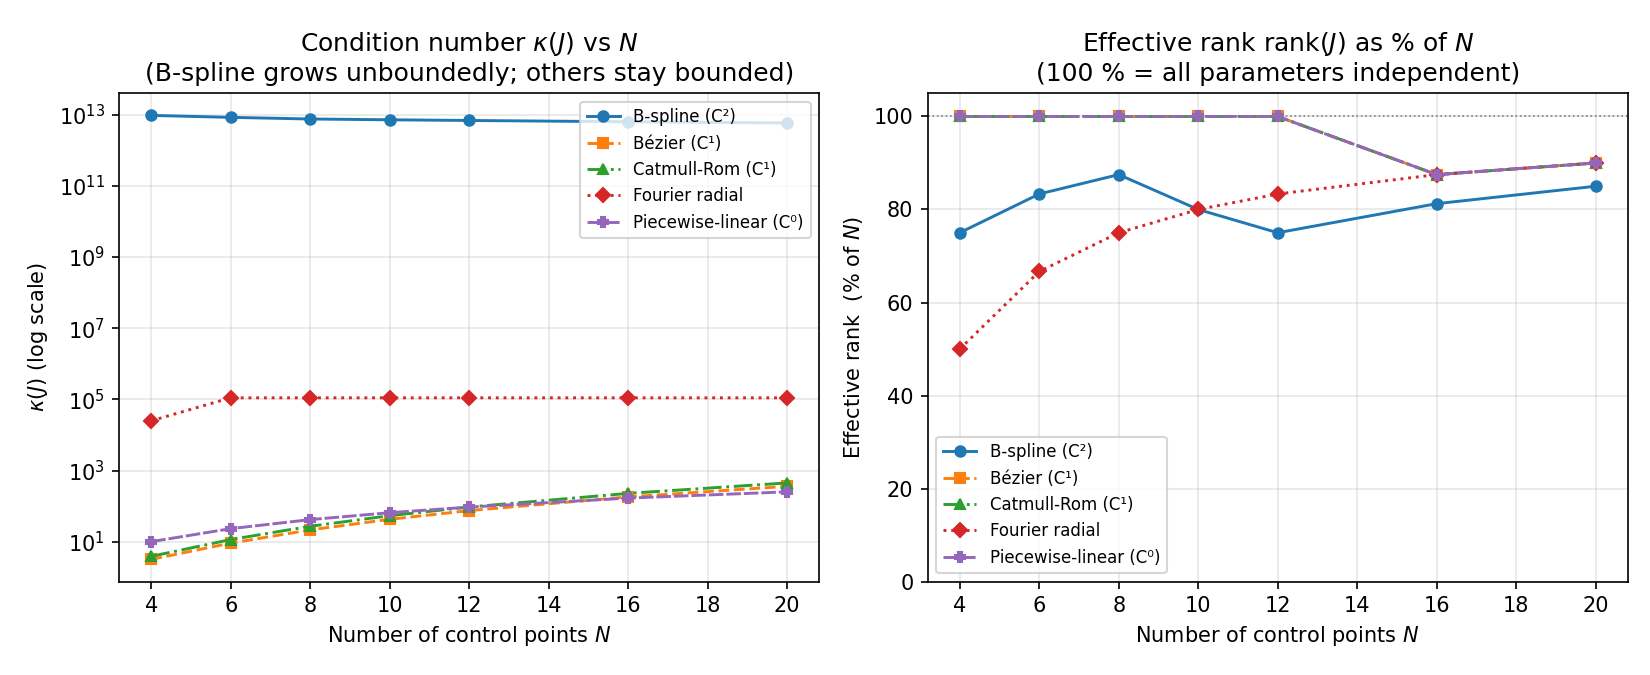
\includegraphics[width=\linewidth]{../docs/figures/stab_cond_vs_N.png}

{\footnotesize
\textit{Fig.~6:} $\kappa(J)$ and effective rank vs.\ $N$ control points.
B-spline ill-conditioning is structural --- $\kappa{\sim}10^{13}$ at all $N$,
with 15--25\% of parameter directions invisible to mutation.
Bézier and Catmull-Rom remain bounded and full-rank throughout.}

\end{block}

\end{column}

\begin{column}{0.030\paperwidth}\end{column}

% ============================================================
%  COLUMN 4 — Reduced Order Model + Results + Conclusion
% ============================================================
\begin{column}{0.220\paperwidth}

\begin{block}{Reduced-Order Surrogate Model}
\textbf{Motivation:} Fine-mesh FEA ${\approx}300$\,ms/evaluation.
A GP surrogate targets ${\approx}20\times$ speed-up for dense
design-space screening.

\medskip
\textbf{POD stress basis:}
$\widetilde{\mathbf{S}}=\mathbf{U\Sigma V}^\top$;
retain $k$ modes ($\tau{=}95\%$: $k{=}63$; 99\%: $k{=}187$).
Modal coefficients trained via GP regression (one GP per mode).
Safety-factor surrogate: single GP on scalar
$\mathrm{SF}=\sigma_y/\sigma_{\mathrm{VM,max}}$, enabling
$P(\mathrm{SF}{<}1.5)=\Phi\!\left(\tfrac{1.5-\hat{\mu}}{\hat{\sigma}}\right)$
for Bayesian feasibility screening.

\medskip
\textbf{UCB acquisition:}
$a(\boldsymbol{\theta})=\hat{E}_{\text{score}}+\beta\hat{\sigma}$

\medskip
\includegraphics[width=\linewidth]{./assets/mode_shapes.png}

{\footnotesize
\textit{Fig.~7:} First four POD stress basis functions (von-Mises, 2$\times$2).
Mode~1 captures 23.8\% of stress-field variance; modes~1--4 collectively
explain ${>}50\%$, motivating the low-rank GP surrogate.}

\medskip
\includegraphics[width=\linewidth]{assets/gp_fit.png}

{\footnotesize
\textit{Fig.~8:} GP predicted vs.\ true modal coefficient for modes~1--4
(trained on $N{=}50$ FEA designs): $R^2\geq0.906$.
Calibration degrades beyond mode~30, motivating active-learning
expansion toward constraint boundaries.}
\end{block}

\begin{block}{Conclusions}
\begin{itemize}\compactlist
  \item \textbf{Catmull-Rom / B\'ezier:} $\kappa(J){<}100$, full rank,
        $\bar{c}{=}1.0$ --- preferred parametrisation for DE
  % \item \textbf{FEA-in-loop} correctly rejects structural failures the
        % formula baseline silently accepts; essential for bar and thin
        % cross-section geometries
  \item \textbf{Energy transfer objective}
        $E_{\text{transfer}}\propto I\omega^2\cos^2\!\theta_c\cdot b/b_{\max}$
        unifies eval in one objestctive physical metric 
  \item \textbf{Surrogate:} 3.9\% LOO peak-stress error at $N{=}50$;
        UCB acquisition targets constraint boundary for efficient expansion
  \item \textbf{Future work:} Experimental validation of design;
        constraint-boundary seeding; improved ROM surrogate. 
\end{itemize}
\end{block}

\end{column}

\begin{column}{0.015\paperwidth}\end{column}
\end{columns}
\end{frame}
\end{document}
